\documentclass{article}
\usepackage{icmcsmc2014}
\usepackage{times}
\usepackage{ifpdf}
\usepackage[english]{babel}
%\usepackage{cite}
\usepackage{fancyvrb}
%%%%%%%%%%%%%%%%%%%%%%%% Some useful packages %%%%%%%%%%%%%%%%%%%%%%%%%%%%%%%
%%%%%%%%%%%%%%%%%%%%%%%% See related documentation %%%%%%%%%%%%%%%%%%%%%%%%%%
%\usepackage{amsmath} % popular packages from Am. Math. Soc. Please use the 
%\usepackage{amssymb} % related math environments (split, subequation, cases,
%\usepackage{amsfonts}% multline, etc.)
%\usepackage{bm}      % Bold Math package, defines the command \bf{}
%\usepackage{paralist}% extended list environments
%%subfig.sty is the modern replacement for subfigure.sty. However, subfig.sty 
%%requires and automatically loads caption.sty which overrides class handling 
%%of captions. To prevent this problem, preload caption.sty with caption=false 
%\usepackage[caption=false]{caption}
%\usepackage[font=footnotesize]{subfig}


%user defined variables
\def\papertitle{Advances in Modality}
\def\firstauthor{First author}
\def\secondauthor{Second author}
\def\thirdauthor{Third author}


% authors so far:
% AdC, Till, Jeff, Miguel

% adds the automatic
% Saves a lot of ouptut space in PDF... after conversion with the distiller
% Delete if you cannot get PS fonts working on your system.

% pdf-tex settings: detect automatically if run by latex or pdflatex
\newif\ifpdf
\ifx\pdfoutput\relax
\else
   \ifcase\pdfoutput
      \pdffalse
   \else
      \pdftrue
\fi

\ifpdf % compiling with pdflatex
  \usepackage[pdftex,
    pdftitle={\papertitle},
    pdfauthor={\firstauthor, \secondauthor, \thirdauthor},
    bookmarksnumbered, % use section numbers with bookmarks
    pdfstartview=XYZ % start with zoom=100% instead of full screen; 
                     % especially useful if working with a big screen :-)
   ]{hyperref}
  %\pdfcompresslevel=9

  \usepackage[pdftex]{graphicx}
  % declare the path(s) where your graphic files are and their extensions so 
  %you won't have to specify these with every instance of \includegraphics
  \graphicspath{{./figures/}}
  \DeclareGraphicsExtensions{.pdf,.jpeg,.png}

  \usepackage[figure,table]{hypcap}
\fi

%setup the hyperref package - make the links black without a surrounding frame
\hypersetup{
    colorlinks,%
    citecolor=black,%
    filecolor=black,%
    linkcolor=black,%
    urlcolor=black
}


% Title.
% ------
\title{\papertitle}

% Authors
% Please note that submissions are NOT anonymous, therefore 
% authors' names have to be VISIBLE in your manuscript. 
%
% Single address
% To use with only one author or several with the same address
% ---------------
%\oneauthor
%   {\firstauthor} {Affiliation1 \\ %
%     {\tt \href{mailto:author1@smcnetwork.org}{author1@smcnetwork.org}}}

%Two addresses
%--------------
% \twoauthors
%   {\firstauthor} {Affiliation1 \\ %
%     {\tt \href{mailto:author1@smcnetwork.org}{author1@smcnetwork.org}}}
%   {\secondauthor} {Affiliation2 \\ %
%     {\tt \href{mailto:author2@smcnetwork.org}{author2@smcnetwork.org}}}

% Three addresses
% --------------
 \threeauthors
   {\firstauthor} {Affiliation1 \\ %
     {\tt \href{mailto:author1@smcnetwork.org}{author1@smcnetwork.org}}}
   {\secondauthor} {Affiliation2 \\ %
     {\tt \href{mailto:author2@smcnetwork.org}{author2@smcnetwork.org}}}
   {\thirdauthor} { Affiliation3 \\ %
     {\tt \href{mailto:author3@smcnetwork.org}{author3@smcnetwork.org}}}


% ***************************************** the document starts here ***************
\begin{document}
%
\capstartfalse
\maketitle
\capstarttrue
%
\begin{abstract}
	Modality is a toolkit to improve and facilitate the use of digital technology within sound art and music, based on the audio programming language SuperCollider.
\end{abstract}

\begin{figure}[h]
	\centering
		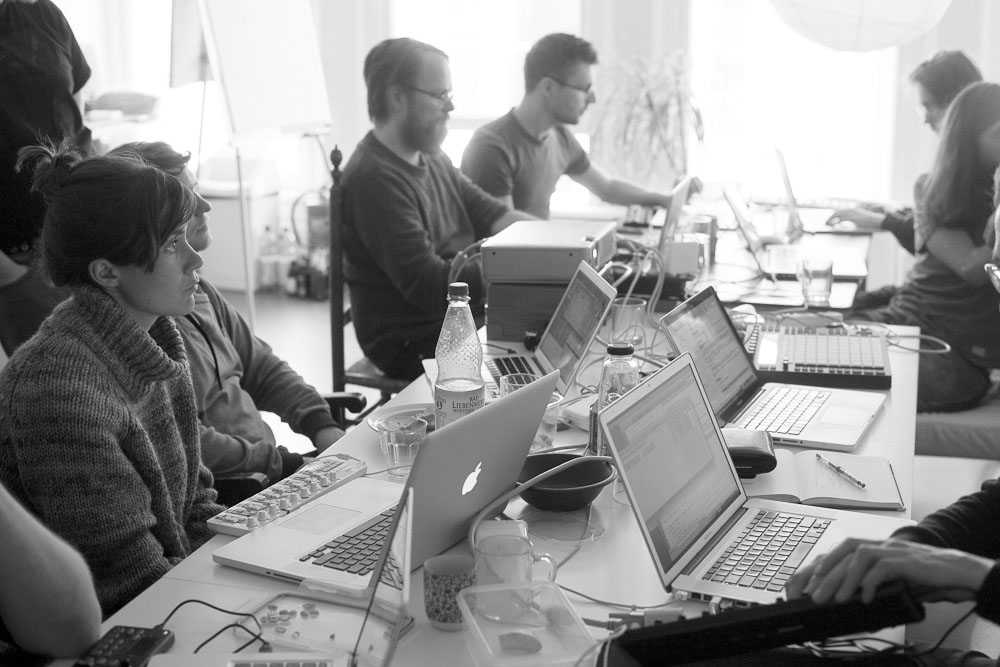
\includegraphics[width=.9\columnwidth]{../media/20140331-IMG_5976.jpg}
	\caption{Meeting 2014 in Amsterdam}
	\label{fig:media_20140331-IMG_5976}
\end{figure}

\section{Overview of the modality concept and its aims}
\label{sec:overview_of_modality_concept_and_aims}


Modality is a project dedicated to modal interaction with synthesis processes for physical control in performance. Its primary product is the Modality Toolkit, a library to facilitate straightforward access to hardware controllers in the SuperCollider programming language. It is designed and developed by the ModalityTeam, a group of people that see themselves as both users and developers both of and for SuperCollider.

The idea behind the Modality Toolkit is to simplify the creation of individual electronic instruments using controllers of various kinds. 
To this end, a common code interface, MKtl, is used for connecting controllers from various sources and protocols. 
Currently HID and MIDI are supported with OSC, GUI-based interfaces can be created on the fly from interface descriptions.


\section{Scope of Modality}
\label{sec:scope_of_modality_tech_info_where_what}

\emph{Tells about the scope of the modality group, how it was established and how the meetings work. Should especially include a description of the combination of developer meeting, public workshop and concert.}

The name Modality arose from the idea to scaffold the creation of modal interfaces, i.e., to create interfaces where e.g. one physical controller can be used for different purposes or it is possible to switch its functionality, even at runtime. It is our belief that integration of such on-the-fly remapping features helps to create instruments that are flexible, powerful, and interesting to play. The strength of such a modal interface is that it allows for fast changes and more opportunity for sonic discovery as can be necessary when, for example, improvising with musicians playing acoustic instruments. 


\subsection{Unifications of interface implementations}
\label{sub:unifications_of_interface_implementations}

With MKtl, it is possible to assign functionality to controller elements.  A control element is a part of a controller that generates a one-dimensional stream of events, accepts a one-dimensional stream of events or both of the above.

Each MKtl object has elements such as sliders or knobs. It is possible to assign an action to such an element that is evaluated every time the value of that element gets updated. 

 Below, there are two examples using a popular MIDI controller.

\begin{Verbatim}
k = MKtl('nnkn20');
\end{Verbatim}



\begin{itemize}
	\item Modality toolkit + Various Mixed Things + closely related
	\item more related libs - FP/FRP, wslib, JITLibExtensions, 
		all of Marijes device related quarks, etc 
\end{itemize}

\begin{figure}[h]
	\centering
		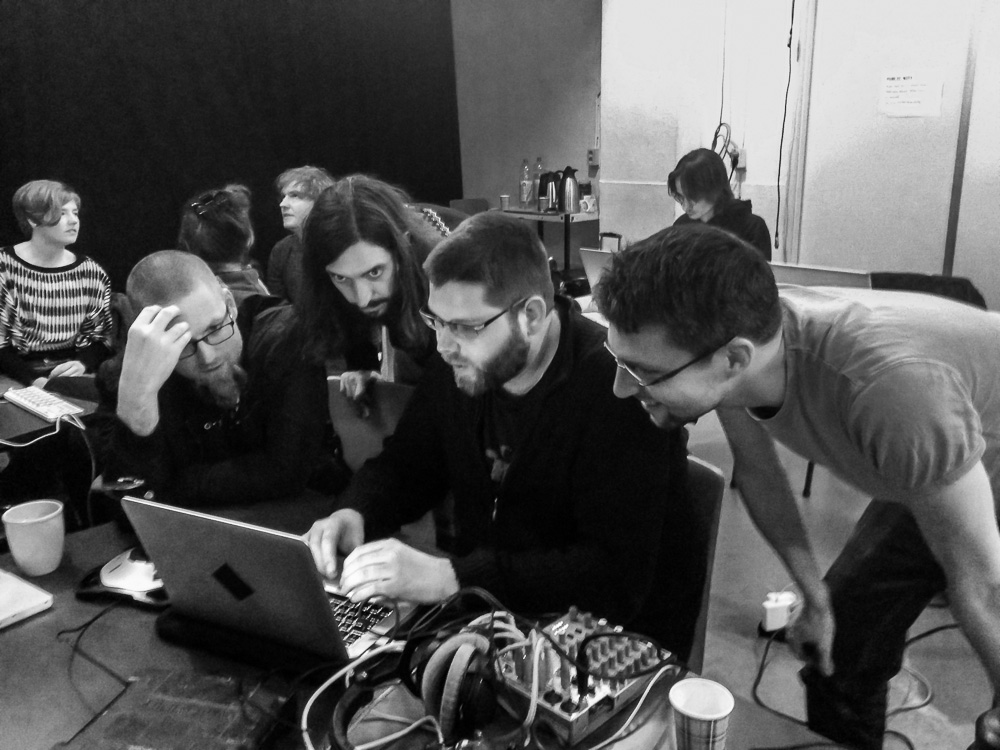
\includegraphics[width=.9\columnwidth]{../media/20140403-IMG_1667.jpg}
	\caption{Public workshop and open Lab at STEIM}
	\label{fig:media_20140331-IMG_5976}
\end{figure}


\section{Description files}
\label{sec:descriptions_files}

In order for Modality to be able to use a device a \textit{device description} file must be available for it.  A device description file characterizes and labels each element and provides the shape of the data structure used to access elements. It is implemented using one text file per device containing an sclang dictionary with (at least) fields 'protocol' (only one protocol allowed per device, currently only HID and MIDI implemented), 'device' (the operating system provided name of the device) and 'description'. The 'description' field contains a dictionary with a tree-like structure, where the value at each key can be another dictionary or array and where the leafs contain a dictionary describing each element. These element dictionaries contain the technical specifications of the element, namely identification information (e.g. for MIDI, the MIDI number and channel), the physical type of control (button, slider, e.t.c.) and a \textit{ControlSpec} that specifies how to convert the incoming values to the range $[0,1]$.   \emph{Slould we include the ABNF definition  in an annex ? point to it online ?} Following is the element dictionary for a button of a MIDI device.

\begin{Verbatim}
\rew: (
	\midiMsgType: \cc,
	\type: \button,
	\midiChan: 0,
	\midiNum: 47,
	\spec: \midiBut,
	\mode: \push
)
\end{Verbatim}

Elements which are physically (or virtually) grouped on the device such as with pages, rows or columns are grouped together in the description file using arrays. For instance the third button on the second row of page 4 of a Korg NanoKONTROL can be accessed with the following code:

\begin{Verbatim}
MKtl('nnkn0').elements[\sl][3][1][2]
\end{Verbatim}

The hierarchical grouping of elements also facilitates bulk addressing of elements by traversing the hierarchy starting at the desired node. For instance, it's easy to programatically add actions to multiple elements:

\begin{Verbatim}
MKtl('nnkn0').elements[\sl]
.do{ |xs, page|
 xs.do{ |xs, row|
  xs.do{ |element, column|
   element.action = 
    {[page, row, column].postln}
  }
 }
}
  		
\end{Verbatim}

The standard order for grouped elements is first page, then row starting from the top of controller and finally column starting from the left of the controller.

New devices can be added to modality easily, all that is needed is to write the corresponding device description file. If a user tries to access a device for which there is still no description file available the toolkit can help the user with the creation of the description file. For HID devices a description file can be generated using the HIDExplorer class from the information provided by the HID stack at the operating system level. For MIDI devices the user is asked to press or move all the physical controls available and then a description file is generated with the recorded data. In both cases the user should then supply suitable labels or placement in an array for each element, and complete or correct the information provided.





\section{Islands and Bridges, uniform protocols}
\label{sec:islands_and_bridges_uniform_protocols}



\subsection{ Uniform devices (MIDI, HID, OSC, GUI, Serial) }

		with rich descriptions, hierarchical names for all elements
		FakeGUI for everything


\subsection{ Uniform destinations}

		set messages, RelSet, SoftSet, // if Influx, influence

\emph{ miguel: I'm a bit skeptical about us really having a uniform protocol for destinations. MKtl allows registering call-backs for actions, so does Influx, etc, ok, but so do the stock SC guis, MIDIFunc, etc.  I wonder if we are not claiming too much by saying we have created uniform protocols when all that we are doing is providing call-backs which are known and used everywhere in SuperCollider. One could argue all of Supercollider uses a uniform protocol which is calling methods on objects. Maybe I'm missing something here.
}
 
		
\begin{figure}[h]
	\centering
		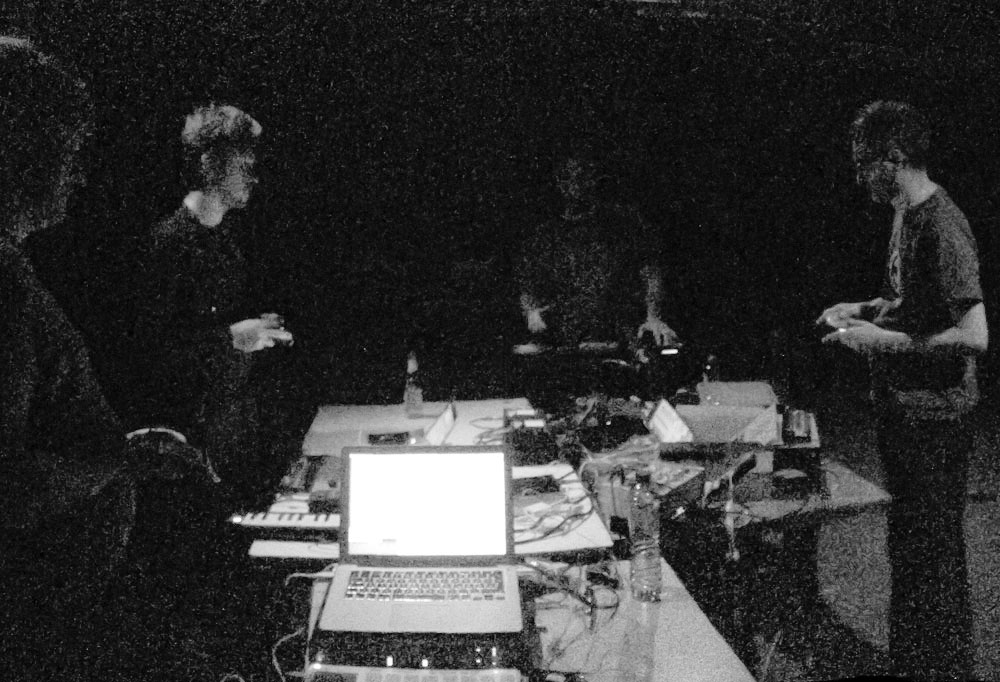
\includegraphics[width=.9\columnwidth]{../media/20140405-IMG_1691.jpg}
	\caption{Modality Concert 2014 at OT301}
	\label{fig:media_20140405-IMG_1691}
\end{figure}

\subsection{Transformer islands} 

What are they supposed to be ? Why are there several different ones ?	
	
\subsubsection{MDispatch}	

describe : An initial attempt, interesting but didn't catch on.
		
\subsubsection{FRP}

describe~\cite{-uni}



\subsubsection{Influx}

describe

\subsubsection{others}

which ones ?

\section{Examples / Use Cases}
\label{sec:examples_use_cases}


\subsection{MPD 18}
\label{sub:mpd_18}

The MPD18 has 16 Buttons and a slider.

    [Sound Buttons] Buttons 1-3 are mapped to adsr enveloped sound sources.
        By pushing them down sound turns on; releasing: sound off.
    the Slider sets amplitude (or pitch) for the (sound)source of the currently depressed button.
    [Memory Slots] Buttons 5-16 represent 'memory' positions (initially not mapped)
        if sound is assigned (see below), sound is played when button depressed.
    [Shift Button] Button 4 is a 'shift key'. When depressed
        Sound Buttons don't trigger any sound but select the active slot. This can be followed by
        depressing a Memory Slot button, which assigns the selected sound to that pad.
        if you release the shift key before assignment, nothing happens.
        assigning a copy to an already assigned memory slot replaces existing
        mute copy +[Sound Button then Shift button]
        Sound Button triggers sound
        depress Memory Slot button, assigning the sound to the pad, with sound

\subsection{Switching actions}
\label{sub:switching_actions}

Switching actions from one controller to another mid-way through a performance.

\subsection{An example of a performance setup with influx and KtlLoop}

\emph{Would this make sense here ?}

\section{Conclusions}
\label{sec:conclusions}



Claims to originality:
* incoming data is associated with a rich knowledge of what generated it. possible to query elements based on type.
* access to elements done in a logical and memorize-able way, both through the auto-generated device names and element hierarchy.
* automatic initialization reduces startup to one line of code.
* Uniform access to controls from devices across multiple controllers and protocols.
* Several ways to take inputs and create complex instruments investigated.

We have showed beyond doubt that Modality is the best thing since sliced bread. It surpasses all other solutions out there both already invented and to be invented in the future. Resistance is futile, you will modalidated.


\begin{acknowledgments}
The Modality team is (in alphabetical order):
    Marije Baalman,
	Tim Blechmann,
    Till Bovermann,
    Alberto de Campo,
    Jeff Carey,
    Bjoernar Habbestad,
	Dominik Hildebrand Marques Lopes,
	Amelie Hinrichsen,
    Robert van Heumen,
    Hannes Hoelzl,
    Miguel Negrao, and
    Wouter Snoei.
Associated organisations are (in alphabetical order):
BEK,
the project \emph{Design, Development and Dissemination of New Musical Instruments} of UdK Berlin/TU Berlin, supported by the Einstein Foundation,
nescivi, and
STEIM.



\end{acknowledgments} 

%%%%%%%%%%%%%%%%%%%%%%%%%%%%%%%%%%%%%%%%%%%%%%%%%%%%%%%%%%%%%%%%%%%%%%%%%%%%%
%bibliography here
\bibliography{icmcmodality}

\end{document}
